\subsection*{Partie I - Définition et propriétés.}
\begin{enumerate}
 \item
\begin{enumerate}
 \item La linéarité est évidente avec les opérations polynomiales.
 \item Si $u$ est bijective, elle est en particulier surjective et le polynôme $1$ est une image par $u$. Il existe donc des polynômes $A$ et $B$ tels que $1=PA + QB$ ce qui entraine $P$ et $Q$ premiers entre eux d'après le théorème de Bezout.
 \item Supposons $P$ et $Q$ premiers entre eux et considérons $(A,B)\in \ker u$.\newline
Alors $PA = -QB$ donc $P$ divise $QB$. Or $P$ est premier avec $Q$ donc $Q$ divise $B$ d'après le théorème de Gauss. Comme $A,B)\in E$, le degré de $B$ est strictement plus petit que celui de $Q$. On doit donc avoir $B=0$ ce qui entraine $A$ nul et l'injectivité de $u$.\newline
Comme $u$ est une application linéaire entre deux espaces vectoriels de \emph{même} dimension, on en déduit que $u$ est bijective.
\end{enumerate}
 
 \item
\begin{enumerate}
 \item Par définition, $\Mat_{\mathcal{B} \mathcal{B}'}u$ est la matrice présentée dans l'énoncé et dont le déterminant est le résultant.
 \item L'application $u$ est bijective si et seulement si $\Mat_{\mathcal{B} \mathcal{B}'}u$ est inversible si et seulement si $\text{Res}(P,Q)\neq 0$.\newline
\emph{Attention} à ne surtout pas parler de $\det u$ qui n'a aucun sens car $u$ \emph{n'est pas} un endomorphisme.\newline
D'autre part, $u$ bijective est équivalent à $P$ et $Q$ premiers entre eux d'après la question 1. Comme on considère des polynômes à coefficients complexes, ils sont scindés. Deux polynômes sont premiers entre eux si et seulement si ils n'ont pas de racine en commun. Deux polynômes ont une racine en commun si et seulement si ils ne sont pas premiers entre eux c'est à dire si et seulement si leur résultant est nul.
\end{enumerate}

 \item
\begin{enumerate}
 \item Un polynôme $P$ à coefficients complexes admet une racine multiple si et seulemnt si il a une racine en commun avec son polynôme dérivé ce qui est équivalent à $\text{Res}(P,P')= 0$.
 \item Soit $P=X^3+aX+b$. Alors $P'=3X^2+a$ et
\begin{displaymath}
 \text{Res}(P,P')=
\begin{vmatrix}
b & 0 & a & 0 & 0 \\
a & b & 0 & a & 0 \\
0 & a & 3 & 0 & a \\
1 & 0 & 0 & 3 & 0 \\
0 & 1 & 0 & 0 & 3 
\end{vmatrix}
\end{displaymath}
Calculons ce déterminant par la méthode du pivot:
\begin{multline*}
 \text{Res}(P,P')=
\begin{vmatrix}
1 & 0 & 0 & 3 & 0 \\
0 & 1 & 0 & 0 & 3 \\
b & 0 & a & 0 & 0 \\
a & b & 0 & a & 0 \\
0 & a & 3 & 0 & a \\
\end{vmatrix}
=
\begin{vmatrix}
1 & 0 & 0 & 3 & 0 \\
0 & 1 & 0 & 0 & 3 \\
0 & 0 & a & -3b & 0 \\
0 & b & 0 & -2a & 0 \\
0 & a & 3 & 0 & a \\
\end{vmatrix} \\
=
\begin{vmatrix}
1 & 0 & 0 & 3 & 0 \\
0 & 1 & 0 & 0 & 3 \\
0 & 0 & a & -3b & 0 \\
0 & 0 & 0 & -2a & -3b \\
0 & 0 & 3 & 0 & -2a \\
\end{vmatrix}
=
\begin{vmatrix}
 a & -3b & 0 \\
 0 & -2a & -3b \\
 3 & 0 & -2a \\
\end{vmatrix}
= a(4a^2)+3(9b^2)\\
= 4a^3+27b^2
\end{multline*}
\end{enumerate}

\end{enumerate}


\subsection*{Partie II - Applications.}
\begin{enumerate}
 \item 
\begin{enumerate}
 \item On calcule le résultant des deux polynômes qui est le déterminant d'une matrice (notons la $A$) $7\times 7$.
\begin{multline*}
 \begin{vmatrix}
1 & 0 & 0 & 1  & 0  & 0  & 0 \\
0 & 1 & 0 & -1 & 1  & 0  & 0 \\
0 & 0 & 1 & 0  & -1 & 1  & 0 \\
1 & 0 & 0 & 1  & 0  & -1 & 1 \\
1 & 1 & 0 & 0  & 1  & 0  & -1 \\
0 & 1 & 1 & 0  & 0  & 1  & 0 \\
0 & 0 & 1 & 0  & 0  & 0  & 1
 \end{vmatrix}
=
 \begin{vmatrix}
1 & 0 & 0 & 1  & 0  & 0  & 0 \\
0 & 1 & 0 & -1 & 1  & 0  & 0 \\
0 & 0 & 1 & 0  & -1 & 1  & 0 \\
0 & 0 & 0 & 0  & 0  & -1 & 1 \\
0 & 1 & 0 & -1 & 1  & 0  & -1 \\
0 & 1 & 1 & 0  & 0  & 1  & 0 \\
0 & 0 & 1 & 0  & 0  & 0  & 1
 \end{vmatrix} \\
=
 \begin{vmatrix}
 1 & 0 & -1 & 1  & 0  & 0 \\
 0 & 1 & 0  & -1 & 1  & 0 \\
 0 & 0 & 0  & 0  & -1 & 1 \\
 1 & 0 & -1 & 1  & 0  & -1 \\
 1 & 1 & 0  & 0  & 1  & 0 \\
 0 & 1 & 0  & 0  & 0  & 1
 \end{vmatrix}
=
 \begin{vmatrix}
 1 & 0 & -1 & 1  & 0  & 0 \\
 0 & 1 & 0  & -1 & 1  & 0 \\
 0 & 0 & 0  & 0  & -1 & 1 \\
 0 & 0 & 0  & 0  & 0  & -1 \\
 0 & 1 & 1  & -1 & 1  & 0 \\
 0 & 1 & 0  & 0  & 0  & 1
 \end{vmatrix}\\
= -
 \begin{vmatrix}
 1 & 0  & -1 & 1   \\
 0 & 0  & 0  & -1  \\
 1 & 1  & -1 & 1   \\
 1 & 0  & 0  & 0  
 \end{vmatrix}
=
 \begin{vmatrix}
 1 & 0  & -1  \\
 1 & 1  & -1  \\
 1 & 0  & 0   
 \end{vmatrix}
=
 \begin{vmatrix}
0  & -1  \\
1  & -1  \\
 \end{vmatrix} = 1
\end{multline*}
Comme ce résultant est non nul, les polynômes sont premiers entre eux.
 \item D'après la première partie, on peut trouver le couple $(A,B)$ en résolvant l'équation vectorielle
\begin{displaymath}
 u(A,B)=1
\end{displaymath}
Elle se traduit par l'équation matricielle $AX=C$ où $X$ est une matrice colonne inconnue à 7 lignes et $C$ la matrice colonne dont le premier coefficient vaut $1$ et les autres $0$.\newline
Les trois premières lignes donnent les coefficients de $A_0$ et les quatre dernières celles de $B_0$. Notons $x_1,\cdots, x_7$ les coefficients de $X$.\newline
Résolvons le système associé à cette équation matricielle par une méthode du pivot :
\begin{multline*}
AX = C  
\Leftrightarrow
 \left\lbrace 
\begin{aligned}
 &x_1 &     &     &+x_4 &     &     &     &= 1\\ 
 &    &x_2  &     &-x_4 &+x_5 &     &     &= 0\\
 &    &     &x_3  &     &-x_5 &+x_6 &     &= 0\\
 &x_1 &     &     &x_4  &     &-x_6 &+x_7 &= 0\\
 &x_1 &+x_2 &     &     &+x_5 &     &-x_7 &= 0\\
 &    &x_2  &+x_3 &     &     &+x_6 &     &= 0\\
 &    &     &x_3  &     &     &     &+x_7 &= 0
\end{aligned}
\right. \\
\Leftrightarrow
 \left\lbrace 
\begin{aligned}
 &x_1 &      &     &+x_4 &     &     &     &= 1\\ 
 &    &x_2   &     &-x_4 &+x_5 &     &     &= 0\\
 &    &      &x_3  &     &-x_5 &+x_6 &     &= 0\\
 &    &      &     &     &     &-x_6 &+x_7 &= -1\\
 &    &x_2   &     &-x_4 &+x_5  &     &-x_7 &= -1\\
 &    &x_2   &+x_3 &     &     &+x_6 &     &= 0\\
 &    &      &x_3  &     &     &     &+x_7 &= 0
\end{aligned}
\right. \\
\Leftrightarrow
 \left\lbrace 
\begin{aligned}
 &x_1 &      &     &+x_4 &     &     &     &= 1\\ 
 &    &x_2   &     &-x_4 &+x_5 &     &     &= 0\\
 &    &      &x_3  &     &-x_5 &+x_6 &     &= 0\\
 &    &      &     &     &     &-x_6 &+x_7 &= -1\\
 &    &      &     &     &     &     &-x_7 &= -1\\
 &    &      &x_3  &+x_4 &-x_5 &+x_6 &     &= 0\\
 &    &      &x_3  &     &     &     &+x_7 &= 0
\end{aligned}
\right.
\end{multline*}
\begin{multline*}
\Leftrightarrow
 \left\lbrace 
\begin{aligned}
 &x_1 &      &     &+x_4 &     &     &     &= 1  \\ 
 &    &x_2   &     &-x_4 &+x_5 &     &     &= 0  \\
 &    &      &x_3  &     &     &     &+x_7 &= 0  \\
 &    &      &x_3  &     &-x_5 &+x_6 &     &= 0  \\
 &    &      &x_3  &+x_4 &-x_5 &+x_6 &     &= 0   \\
 &    &      &     &     &     &-x_6 &+x_7 &= -1 \\
 &    &      &     &     &     &     &-x_7 &= -1 \\
\end{aligned}
\right. \\
\Leftrightarrow
 \left\lbrace 
\begin{aligned}
 &x_1 &      &     &+x_4 &     &     &     &= 1  \\ 
 &    &x_2   &     &-x_4 &+x_5 &     &     &= 0  \\
 &    &      &x_3  &     &     &     &+x_7 &= 0  \\
 &    &      &     &     &-x_5 &+x_6 &-x_7 &= 0  \\
 &    &      &     &x_4 &-x_5 &+x_6 &-x_7 &= 0   \\
 &    &      &     &     &     &-x_6 &+x_7 &= -1 \\
 &    &      &     &     &     &     &-x_7 &= -1 \\
\end{aligned}
\right.
\Leftrightarrow
\begin{pmatrix}
 x_1 \\ x_2 \\  x_3 \\  x_4 \\  x_5 \\  x_6 \\  x_7 
\end{pmatrix}
=
\begin{pmatrix}
 1 \\ -1 \\  -1 \\  0 \\  1 \\  2 \\  1
\end{pmatrix}
\end{multline*}
On en tire
\begin{displaymath}
 A_0 = 1-X-X^2 \hspace{1cm} B_0 = X + 2X + X^3 
\end{displaymath}

 \item Il s'agit d'une question de cours classique utilisant le théorème de Gauss. Les couples cherchés sont de la forme
\begin{displaymath}
 \left( A_0 + \Lambda B, B_0 - \Lambda A\right) 
\end{displaymath}
où $\Lambda$ est un polynôme quelconque.
\end{enumerate}

% \item
%\begin{figure}[h!t]
% \centering
% 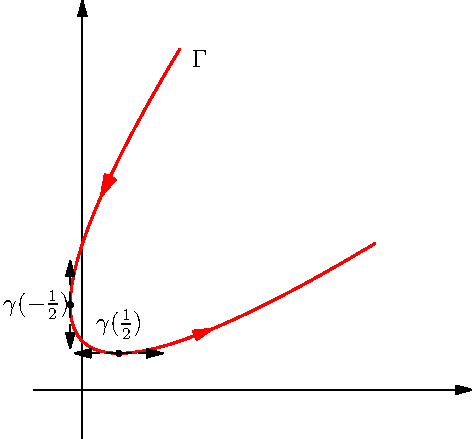
\includegraphics{./Cresult1_1.pdf}
 % Cresult1_1.pdf: 0x0 pixel, -2147483648dpi, 0.00x0.00 cm, bb=
% \caption{Tracé de $\Gamma$}
% \label{fig:Cresult1_1}
%\end{figure}

%\begin{enumerate}
% \item On note $\gamma$ la fonction à valeur dans $\R^2$ dont l'image est $\Gamma$. On ne voit pas de transformation simple conduisant à une symétrie de la courbe. On peut étudier facilement les variations des deux projections sur le axes.\newline
%La courbe admet des branches infinies pour lorsque le paramètre $t$ tend vers $+\infty$ ou -$\infty$. Les fonctions $x$ et $y$ sont alors clairement équivalentes ce qui signifie que la courbe admet $\overrightarrow i + \overrightarrow j $  comme direction asymptotique. La courbe n'admet pas d'asymptote car $x(t)-y(t)=2t-1$ diverge vers $+\infty$ ou $-\infty$.\newline
%Le tracé à la machine est présenté dans la figure \ref{fig:Cresult1_1}. Il ressemble à une parabole, la recherche de l'équation cartésienne  dans la question suivante permettra de montrer que c'est bien une parabole.
% \item Un point $M$ de coordonnées $(x,y)$ appartient à la courbe si et seulement si il existe un $t$ réel tel que $x=P(t)$ et $y=Q(t)$.\newline
%Dans ce cas, les polynômes $A_x$ et $B_y$ ont une racine (réelle) en commun. Il faut noter qu'il pourrait y avoir une racine non réelle en commun. On a donc seulement une implication : $M$ appartient à la courbe entraine $\text{Res}(A_x,B_y)=0$.\newline
%Dans le cas particulier de la question précédente, on doit calculer le résultant des polynômes $X^2+X-x$ et $X^2-X+1-y$. Il vient
%\begin{multline*}
%\begin{vmatrix}
%-x & 0  & 1-y & 0   \\
%1  & -x & -1  & 1-y \\
%1  & 1  & 1   & -1  \\
%0  & 1  & 0   & 1
%\end{vmatrix} 
%=
%\begin{vmatrix}
%1  & 1  & 1   & -1  \\
%-x & 0  & 1-y & 0   \\
%1  & -x & -1  & 1-y \\
%0  & 1  & 0   & 1
%\end{vmatrix} \\
%=
%\begin{vmatrix}
%1  & 1    & 1      & -1  \\
%0  & x    & 1-y +x & -x  \\
%0  & -x-1 & -2     & 2-y \\
%0  & 1    & 0      & 1
%\end{vmatrix} \\
%= \left((1-y+x)(2-y)-2x \right)+\left(-2x+(x+1)(1-y+x) \right)  \\
%= x^2 + y^2 -2xy -4y +3
%\end{multline*}
%Dans ce cas particulier, il existe un moyen beaucoup plus simple pour obtenir l'équation cartésienne. Il suffit d'exprimer $t$ en fonction de $x$ et $y$ pour %un point de la courbe puis de remplacer. On obtient $x-y = 2t-1$ donc 
%\begin{displaymath}
% t = \frac{1}{2}(x-y+1)
%\end{displaymath}
 
% \item L'équation étant du second degré, il s'agit d'une conique. C'est une parabole car son discriminant est nul.
%\end{enumerate}

 \item Considérons des polynômes $P$ et $Q$ avec des ensembles de racines respectivement $\mathcal{R}$ et $\mathcal{S}$. Pour $y$ réel, formons le polynôme $B_y $ obtenu en substituant $y-X$ à $X$ dans $B$.\newline
Pour tout $z\in\C$, $z$ est racine de $Q_y$ si et seulement si $y-z$ est racine de $B$.\newline
On peut alors écrire
\begin{multline*}
\text{Res}(P,Q_y)=0 \Leftrightarrow
 P \text{ et } Q_y\text{ ont une racine en commun} \\
\Leftrightarrow \exists z\in \mathcal{R} \text{ tq } y-z \in \mathcal{S} 
\Leftrightarrow \exists (z,x)\in \mathcal{R}\times\mathcal{S} \text{ tq } y-z = x  \\
\Leftrightarrow \exists (z,x)\in \mathcal{R}\times\mathcal{S} \text{ tq } y = z + x 
\end{multline*}
Comme $\text{Res}(P,Q_y)$ est une expression polynomiale en $y$, les racines du polynômes associé sont donc les sommes des racines des polynômes de départ.\newline
Dans notre cas particulier, on forme encore le résultant
\begin{multline*}
\begin{vmatrix}
3 & 0 & y^2-7 & 0     \\
0 & 3 & -2y   & y^2-7 \\
1 & 0 & 1     & -2y   \\
0 & 1 & 0     &  1
\end{vmatrix}
=
\begin{vmatrix}
1 & 0 & 1     & -2y   \\
3 & 0 & y^2-7 & 0     \\
0 & 3 & -2y   & y^2-7 \\
0 & 1 & 0     &  1
\end{vmatrix} \\
=
\begin{vmatrix}
1 & 0 & 1      & -2y   \\
0 & 0 & y^2-10 & 6y    \\
0 & 3 & -2y    & y^2-7 \\
0 & 1 & 0      &  1
\end{vmatrix}
=
\begin{vmatrix}
1 & 0      &  1    \\
0 & y^2-10 & 6y    \\
3 & -2y    & y^2-7 
\end{vmatrix}
= (y^2-10)^2 + 12 y^2 \\
= y^4 -8y^2 + 100
\end{multline*}

\end{enumerate}
